%%	SECCION documentclass																									 %%	
%%---------------------------------------------------------------------------%%
\documentclass[a4paper]{report}

%%---------------------------------------------------------------------------%%
%%	SECCION usepackage																											 %%	
%%---------------------------------------------------------------------------%%
\usepackage{amsmath, amsthm}
\usepackage[spanish,activeacute]{babel}
\usepackage{caratula}
\usepackage{a4wide}
\usepackage{hyperref}
\usepackage{fancyhdr}
\usepackage{graphicx} % Para el logo magico!
\usepackage{amssymb}
\usepackage{amsmath}
\usepackage[latin1]{inputenc}
\usepackage[dvipsnames,usenames]{color}
\usepackage{amsfonts}
\usepackage{highlight}
\usepackage{marvosym}
\usepackage{subfigure}
\usepackage{pdflscape}
\usepackage{color}
\usepackage{colortbl}
\usepackage{float}

%%---------------------------------------------------------------------------%%
%%	SECCION opciones																												 %%	
%%---------------------------------------------------------------------------%%
\parskip    = 11 pt
\headheight	= 13.1pt
\pagestyle	{fancy}
\definecolor{orange}{rgb}{1,0.5,0}

\addtolength{\headwidth}{1.0in}

\addtolength{\oddsidemargin}{-0.5in}
\addtolength{\textwidth}{1.0in}
\addtolength{\topmargin}{-0.5in}
\addtolength{\textheight}{0.7in}
\definecolor{goldenrod}{rgb}{0.85,0.65,0.13}

\newcounter{usCounter}
\setcounter{usCounter}{1}

\newcommand{\us}[4]{
{\setlength{\arrayrulewidth}{1mm}
\framebox{\parbox{16cm}{
{\textsl{\Large \underline{User story \arabic{usCounter}:}}}
\begin{itemize}
\item \underline{\textbf{Como:}} #1
\item \underline{\textbf{Quiero:}} #2
\item \underline{\textbf{De forma que:}} #3
\end{itemize}
\rule{16cm}{0.2mm}
\underline{\textbf{Story points:}} #4
} } }
\addtocounter{usCounter}{1}}

\newcommand{\specus}[3]{
{\setlength{\arrayrulewidth}{1mm}
\framebox{\parbox{16cm}{
\begin{itemize}
\item \underline{\textbf{Como:}} #1
\item \underline{\textbf{Quiero:}} #2
\item \underline{\textbf{De forma que:}} #3
\end{itemize}
} } }
}


%%---------------------------------------------------------------------------%%
%%	SECCION document	 %%	
%%---------------------------------------------------------------------------%%
\begin{document}
\renewcommand{\chaptername}{Parte }

%%---- Caratula -------------------------------------------------------------%%
\materia{Ingenieria de software 2 (2do cuatrimestre de 2009)}
\titulo{Trabajo Pr�ctico}

\integrante{Elizalde Victoria}{??}{??}
\integrante{Gonzalez, Sergio}{??}{??}
\integrante{Mart'inez, Federico}{17/06}{federicoemartinez@gmail.com}
\integrante{Tleye, Sebastian}{732/05}{stleye@gmail.com}
%\grupo{Grupo ??}
\resumen{
%TODO
}


% TOC, usa estilos locos
\maketitle
\pagestyle{empty}
{
\fancypagestyle{plain}
    {
    \fancyhead{}
    \fancyfoot{}
    \renewcommand{\headrulewidth}{0.0pt}
    } % clear header and footer of plain page because of ToC
\tableofcontents
}

\newpage
% arreglos los estilos para el resto del documento, y
% reseteo los numeros de pagina para que queden bien
\pagenumbering{arabic}
\fancypagestyle{plain} {
    \fancyhead[LO]{Elizalde,Gonzalez, Mart�nez, Tleye}
    \fancyhead[C]{}
    \fancyhead[RO]{P\'agina \thepage\ de \pageref{LastPage}}
    \fancyfoot{}
    \renewcommand{\headrulewidth}{0.4pt}
}
\pagestyle{plain}
\chapter{Introducci�n}
A lo largo de este informe presentaremos el trabajo de implementaci�n realizado para la materia Seguridad de la Informaci�n.

El informe se organiza de la siguiente manera:
\begin{enumerate}
\item Consideraciones generales: Descripci�n general de la aplicaci�n: lenguaje de programaci�n utilizado, modelado de la base de datos, etc.
\item Sniffer: Descripci�n de la implementaci�n del sniffer
\item Reportes: Descripci�n de la herramienta para la generaci�n de reportes
\item Instalaci�n y uso: Documentaci�n sobre como armar el ambiente para utilizar el software y como usarlo
\end{enumerate}

\chapter{Consideraciones generales}
\section{Plataforma}
El trabajo fue realizado y probado en Linux Mint 7: Gloria, el cual esta basado en Ubuntu Jaunty. Creemos que el software deber�a funcionar en otras distribuciones Linux sin problemas, no asi en windows, ya que scapy (una libreria de la cual hablaremos mas adelante) no se encuentra disponible para windows (aunque existe un port\footnote{http://trac.secdev.org/scapy/wiki/WindowsInstallationGuide} que supuestamente brinda casi todas las posibilidades de scapy en windows, no lo probamos).

\section{Lenguaje de programaci�n}
Para la realizaci�n del proyecto utilizamos el lenguaje python, el cual varios miembros del grupo utilizamos. Consideramos que el desarrollo en este lenguaje es sencillo, lo cual permitia que el resto del grupo puede familiarizarse rapidamente con el, ya que no habia un lenguaje manejado por todos.

Las ventaja principal que presenta es justamente que permite una velocidad alta para el desarrollo, sin embargo como contra la performance no es comparable a la que podriamos haber obtenido usando otro lenguaje como por ejemplo C++.

\section{Base de datos}
Para la realizaci�n del trabajo era necesario la utilizaci�n de una base de datos para poder almacenar el tr�fico sniffeado y luego poder analizarlo. Por una cuesti�n de simplicidad se utiliz� el motor sqlite, sin embargo es muy simple de cambiar, a fin de utilizar otro motor mas robusto como puede ser mySQL.

\subsection{SQLAlchemy}
Para facilitarnos la interacci�n con la base de datos decidimos utilizar SQLAlchemy, un ORM para python que es bastante flexible, ademas de simple de utilizar.

Definimos entonces las siguientes clases para hacer el mapeo a la base de datos:
\begin{itemize}
\item MensajeHTTP: Es la clase base de los mensajes HTTP. Posee las caracteristicas generales de los mensajes, ya sean requests, o responses; como pueden ser los headers, el body, direcciones ip o los puertos.
\item RequestHTTP: Subclase de MensajeHTTP, guarda la uri, el metodo y el identificador del response asociado (si corresponde)
\item ResponseHTTP: Subclase de MensajeHTTP, guarda el codigo de respuesta y el mensaje de status
\item RequestNoHTTP: Clase que representa aquellos mensajes sniffeados que no corresponden a trafico HTTP (por ejemplo SSH, o HTTPS) y que provienen desde algun host hacia el proxy.
\item ResponseNoHTTP: Similar a la anterior, pero para los mensajes que provienen del proxy a un host de la red.
\end{itemize}

\begin{figure}[H]
\centering
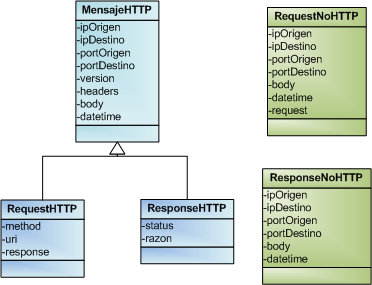
\includegraphics[scale=1]{./figuras/persistencia.png}
\caption{Diagrama con las clases que mapean a la base de datos}
\end{figure}

\chapter{Sniffer}
\section{Sniffeo de la red}
La primera parte del trabajo, consisti� en la implementaci�n de un sniffer, el cual deb�a escuchar el tr�fico que se dirige a un proxy y guardar en una base de datos los mensajes HTTP y otros mensajes como ser SSH, SSL, o TLS.

\begin{figure}[H]
\centering
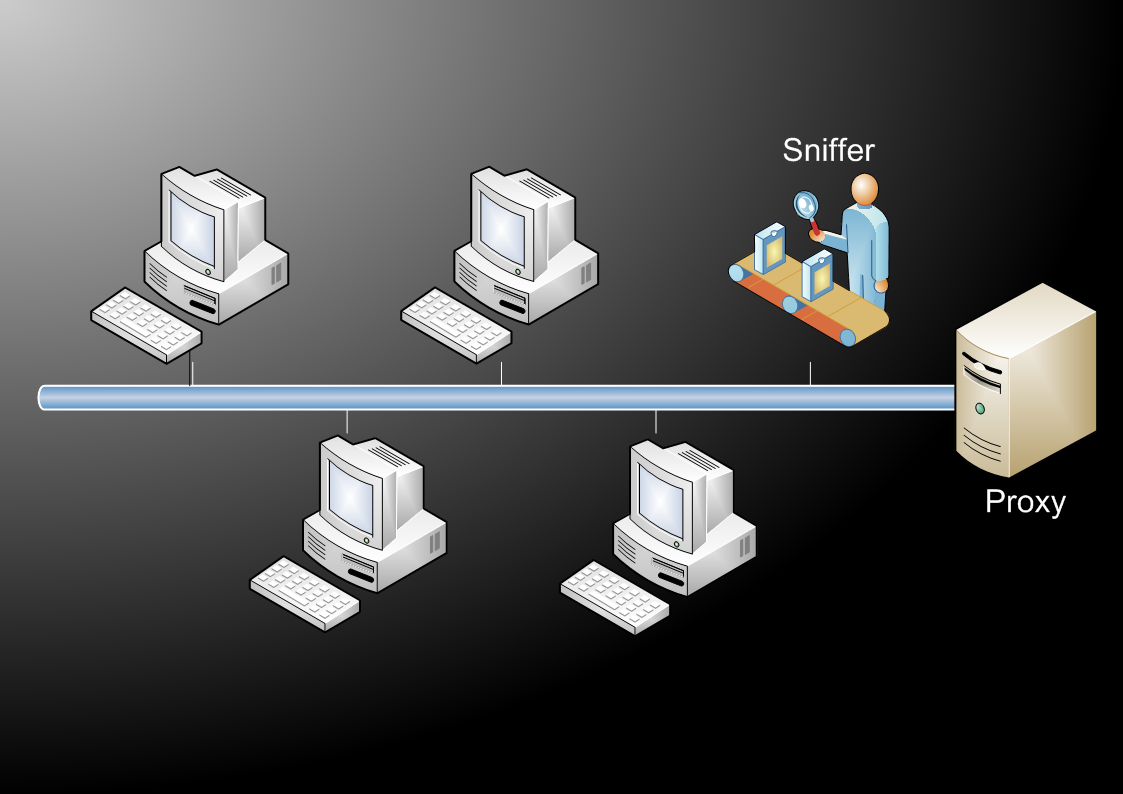
\includegraphics[scale=0.4]{./figuras/sniffer.png}
\caption{Esquema de la ubicaci�n del sniffer}
\end{figure}

Para la construcci�n del sniffer utilizamos la librer�a Scapy. Esta es una librer�a para python que brinda amplias facilidades para el manejo de paquetes a nivel TCP, Ethernet, ICMP y dem�s. Posee ademas otras caracter�sticas interesantes, como la capacidad de generar traceroutes.

Scapy provee una forma de sniffear tr�fico en una interfaz de red. Utilizando esto construimos nuestro sniffer, el cual es capaz de recibir callbacks que se invocan cada vez que se recibe un nuevo paquete. Esta funcionalidad nos permite construir alrededor del sniffer no solo la funcionalidad de capturar y guardar el tr�fico http, sino que permite ademas construir otras funcionalidades que se consideren �tiles. En nuestro caso utilizamos esta posibilidad de los callbacks para realizar dumps a archivos pcap o para ir mostrando por pantalla los paquetes que se iban capturando.

Otra caracter�stica positiva de construir al sniffer de esta manera, es que permite separar el proceso de sniffear del proceso de construir los paquetes HTTP y dem�s, para guardarlos en la base de datos.

El siguiente es un esquema que ilustra la estructura del sniffer:

\begin{figure}[H]
\centering
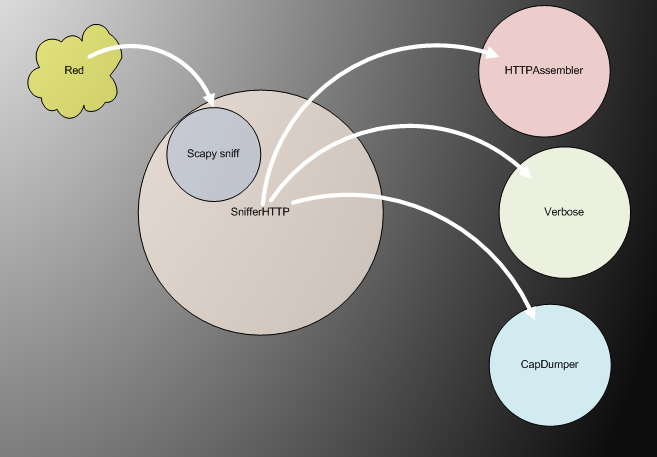
\includegraphics[scale=0.7]{./figuras/esquemaSniff.png}
\end{figure}

En el esquema vemos que utilizando las capacidades de scapy para hacer sniff logramos capturar los paquetes, que luego nuestro sniff pasa a sus suscriptores mediante los callbacks que estos  registran.

\section{Mensajes HTTP}
Cuando se detecta un paquete que llega al puerto del proxy, el mismo pasa a ser examinado. Del paquete se extrae el contenido (o capa RAW), si no hay contenido RAW (por ejemplo se trata de un mensaje TCP SYN) no se procesa. Si el contenido es un mensajeHTTP el mismo se persiste. Si no, se chequea que el mensaje sea el comienzo de un mensaje HTTP y si es as� se crea un estado para la cuadrupla propia de esa conexi�n TCP, donde se van a ir agregando el contenido de los paquetes que lleguen de esa conexi�n, hasta tener el mensaje HTTP completo. Es posible que el mensaje HTTP llegue partido porque TCP no se preocupa por eso sino que es responsabilidad de la aplicaci�n saber cuando terminan sus datos, y como nosotros estamos escuchando la red, vamos a tener que ser nosotros quienes rearmen el mensaje.

Entre los posibles mensajes que se pueden escuchar, hay requests cuyo m�todo  es CONNECT. Estos en general se usan antes de comenzar una conexi�n SSH, TLS, o SSL. Entonces cuando se detecta un CONNECT, se empieza a escuchar ese tr�fico para detectar si se trata de tr�fico no HTTP. En caso afirmativo el tr�fico de la conexi�n se persiste. Notar que a esta altura solo diferenciamos tr�fico HTTP, de tr�fico no HTTP. La discriminaci�n entre otros protocolos de aplicaci�n es posterior.

\section{Otras caracter�sticas de sniffer}
Ademas de sniffear tr�fico HTTP y persitirlo, la aplicaci�n brinda otras funcionalidades, que si bien no fueron pedidas, consideramos que pueden ser �tiles, entre ellas:

\begin{itemize}
\item Dumpeo de la sesi�n de captura a un archivo pcap. Esto es �til si se quiere analizar en otra herramienta las capturas realizadas. El archivo generado contiene todos los paquetes capturados, no solo lo que es tr�fico HTTP.
\item Simulaci�n de una sesi�n de captura a partir de un archivo pcap. El sniffer puede simular una captura en vivo mediante un archivo pcap. Esto es �til si se realizan capturas con otro sniffer como el wireshark, y se desea poder analizar a la misma con la herramienta de reportes que presentaremos mas adelante y que corresponde a la segunda parte del trabajo. Para leer archivos pcaps, tambi�n utilizamos scapy, que nos permite dado un archivo pcap obtener la lista de paquetes que hay en el, sin embargo scapy no preserva las fechas de captura de los paquetes, por lo cual la sesi�n queda guardada en la base de datos, como si se hubiera capturado en vivo en el momento en el que se corri� nuestro sniffer.
\end{itemize}

Ademas, dado que se utiliza un dise�o basado en callbacks, es f�cil extender las funcionalidades del sniffer, simplemente definiendo una clase y suscribiendo un m�todo de la misma que realice las manipulaciones deseada al paquete.

%TODO: tal vez un ejemplo de esto?

\section{Algunas limitaciones}
Nuestro sniffer presenta algunas limitaciones, creemos que las mas importantes son:

\subsection*{Performance}
Si bien creemos que python es un gran lenguaje y muy flexible, somos conscientes que su performance dista de la que se puede lograr programando en C, ademas pudimos averiguar que scapy puede perder paquetes si la carga es muy grande \footnote{http://www.secdev.org/projects/scapy/}. Si bien no pudimos probar al sniffer con una carga muy grande, creemos que es factible que la performance sea un limitante para su uso.

\subsection*{Consideraciones de seguridad}
B�sicamente el sniffer no fue hecho para correr en ambientes hostiles. As� por ejemplo creemos que es factible que un usuario malicioso logre generar una denegaci�n de servicio, generando la ca�da del sniffer. Esto se debe a que como comentamos antes, cuando llega un fragmento de mensaje HTTP se guarda cierta informaci�n de estado para poder armar todo el mensaje. 


\begin{figure}[H]
\centering
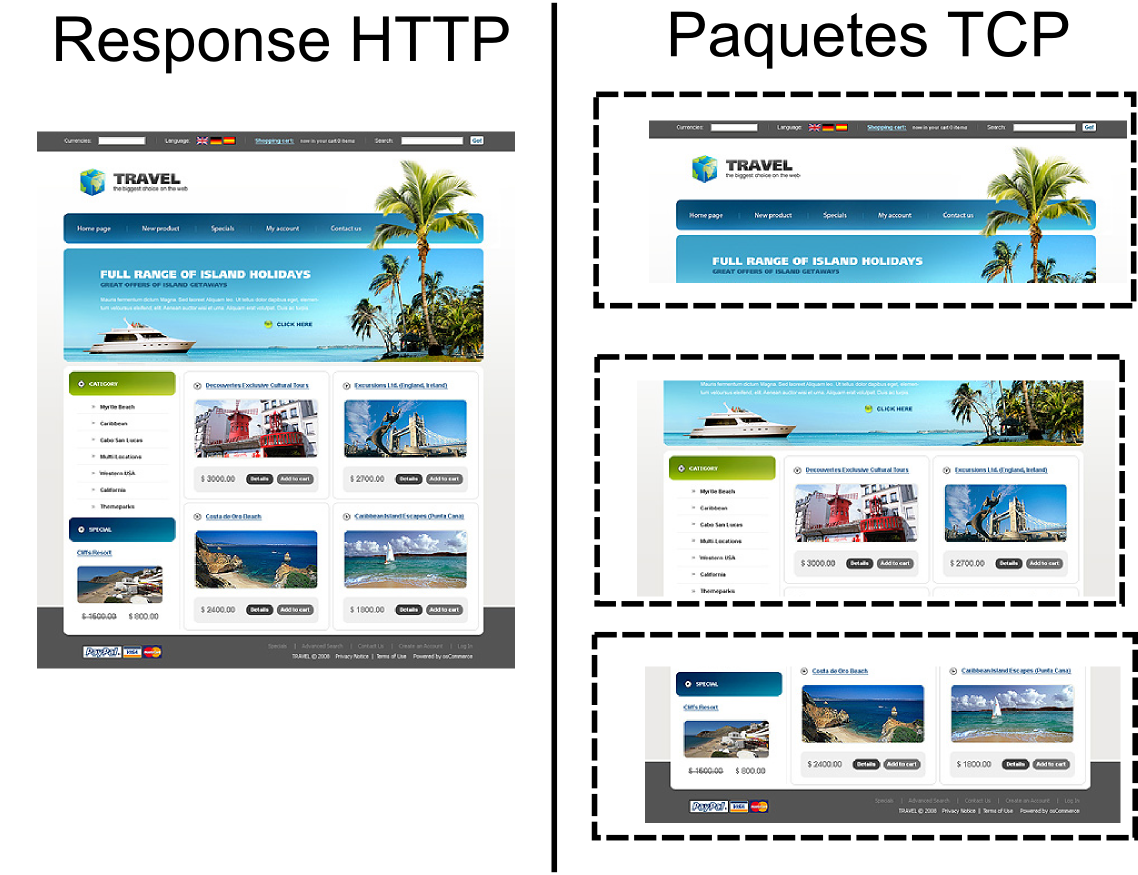
\includegraphics[scale=0.3]{./figuras/fragTCP.png}
\caption{Un mensaje HTTP puede venir fragmentado en varios mensajes TCP}
\end{figure}

Entonces un usuario malicioso puede enviar una gran cantidad de mensajes inconclusos y el sniffer, al guardar la informaci�n de estado de estos, termina agotando sus recursos. Esta situaci�n es similar a lo que ocurre con un ataque de \textit{SYN flooding} en TCP. 

\begin{figure}[H]
\centering
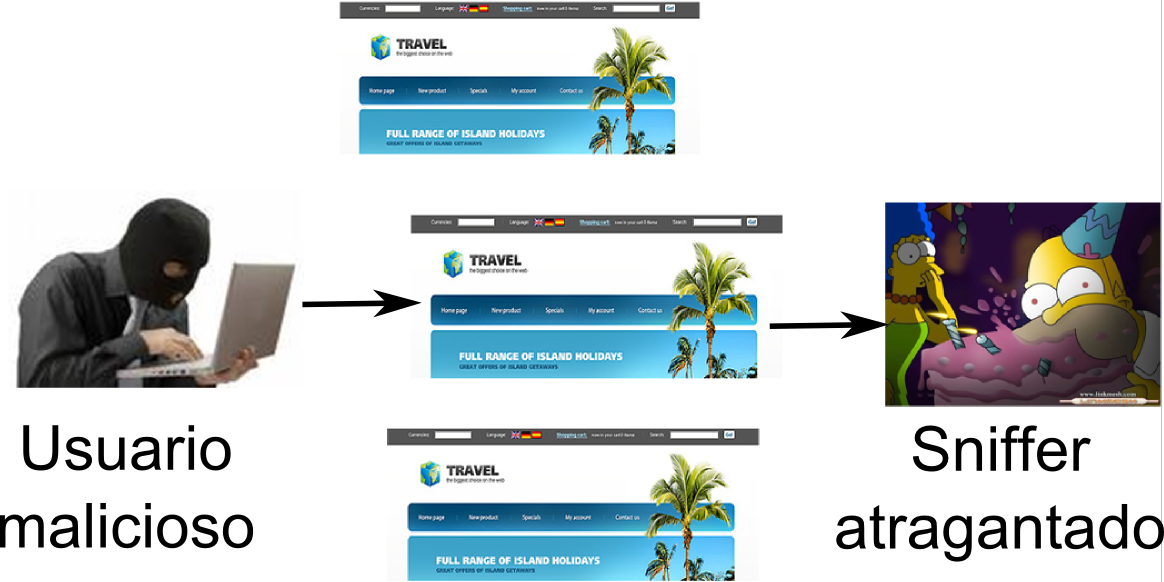
\includegraphics[scale=0.4]{./figuras/atraganta.png}
\caption{Al enviar muchos paquetes inconclusos, un usuario malicioso podr�a lograr agotar los recursos del sniffer}
\end{figure}


Esta vulnerabilidad no fue probada, sin embargo la consideramos altamente factible de explotar.





\chapter{Generaci�n de reportes}
\section{ReporTool}
La segunda parte del trabajo consisti� en la realizaci�n de reportes sobre el tr�fico capturado por el sniffer.
Nosotros construimos una herramienta que denominamos reporTool. La misma permite realizar los distintos analisis de trafico (reportes) generando una salida en formato pdf o en formato html mediante una interfaz grafica.

\begin{figure}[H]
\centering
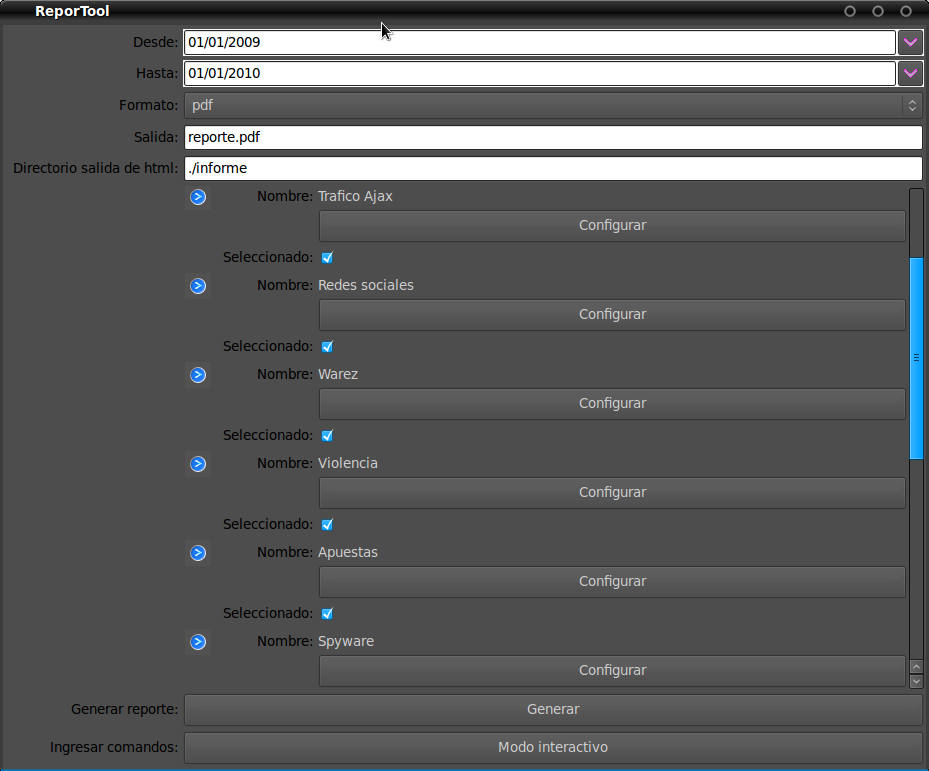
\includegraphics[scale=0.4]{./figuras/Pantallazo.png}
\caption{Captura de pantalla de reporTool}
\end{figure}

En las siguientes secciones daremos una breve descripci�n de los reportes por nosotros realizados. Posteriormente explicaremos el modo interactivo que presenta la herramienta y finalmente mostraremos como es posible agregar reportes propios para ser corridos con reporTool.

\section{Reportes}
Los siguientes son los reportes incluidos con reporTool

\subsection{Reporte de horario laboral}
Este reporte permite analizar el tr�fico discriminandolo seg�n un periodo laboral (d�as de la semana, y rango horario). De esta manera el reporte puede mostrar que usuarios usaron internet fuera de dichos horarios y que porcentaje de su actividad estuvo en infracci�n. El reporte puede mostrar todos los pedidos que se realizaron fuera de horar o solo mostrar el porcentaje en infracci�n.

Ademas puede mostrar la distribuci�n del uso de internet a lo largo de las distintas horas del d�a.

\subsection{Reporte por blacklists}
Este reporte permite especificar en un archivo una lista negra con dominios. El reporte analiza el trafico buscando visitas a alguno de esos dominios. Es en verdad una familia de reportes, ya que es posible utilizar varias instancias del mismo utilizando distintas blacklists, con distintos tipos de dominios, por ejemplo sitios de apuestas, de warez, etc. 

Si bien reporTool trae unos archivos de blacklists para ciertas categorias, es f�cil modificar esas blacklist, o reemplazarlas por otras, crear un reporte nuevo que trabaje con blacklists de otras categorias.

Estas son las blacklists inclu�das con reporTool:
%TODO: listar las blackslists que se incluyen en la entrega

Los siguientes son sitios donde es posible descargar blacklists de distintas categorias:
\begin{itemize}
\item \verb_http://squidguard.mesd.k12.or.us/_
\item \verb_http://www.shallalist.de/_
\item \verb<http://cri.univ-tlse1.fr/documentations/cache/squidguard_en.html#contrib<
\item \verb_http://urlblacklist.com/?sec=download_
\end{itemize}

Este reporte puede generar graficos de cantidad de infracciones por usuarios, que porcenteja del trafico por usuario y total esta en infracci�n, cuales son los sitios de la blacklist mas visitados, entre otras cosas.

\subsection{Reporte de tr�fico AJAX}
%TODO: sergio completa esto

\subsection{Reporte por content type}
%TODO: tleye completa esto

\subsection{Reporte por tr�fico de nivel de aplicaci�n}
%TODO: victoria complete esto por favor :D

\subsection{Reporte de tr�fico global}
%TODO: sergio completa esto, o si queres lo hago yo, pero comete un paty

\subsection{Reporte de seguimiento}
Este reporte permite elegir hasta 5 sitios y analizar la evoluci�n de la cantidad de visitas y de trafico mes a mes para estos sitios, a lo largo de un periodo de tiempo determinado.

\subsection{Reporte por heuristica}
Este reporte puede pensarse de alguna forma como un complemento para el reporte por blacklists. El mismo utiliza un archivo donde se definen ciertas keywords (por ejemplo, keywords sobre apuestas: poker, black jack, casino, etc) que son buscadas en las requests y en los responses. El reporte muestra luego para que usuarios se encontraron matches, asi como cuales fueron los principales matches.

Las blacklists solo encuentran requests a los dominios en ellos definidos, entonces es factible que un usuario pueda visitar alguna p�gina que no esta en la blacklist pero que deber�a estarlo, o que incluso saltee el chequeo de las blacklists (por ejemplo navegando con la cache de google). La busqueda heuristica permite detectar estas cosas, al costo de posiblemente dar falsos positivos sobre el contenido de las visitas. Sin embargo puede ser una herramienta util para detectar usos indebidos.

\section{Modo interactivo}
Ademas de la posibilidad de realizar reportes, reporTool provee un mecanismo interactivo para realizar consultas a la base de datos. En vez de brindar una interfaz para simplemente ejecutar SQL en la base de datos, lo cual es posible con cualquier cliente de bases de datos; brindamos una consola python con ciertos elementos de alto nivel, brindados por el ORM que permiten interactuar con la base de datos.

Para obtener una sesion, se debe utilizar el comando get\_session. Una vez que tenemos una sesion, podemos realizar queries sobre las clases que mapean a la base de datos (presentadas anteriormente) mediante la interfaz que provee sqlalchemy. 

Para mas informacion se puede consultar:

\begin{itemize}
\item \verb<http://www.sqlalchemy.org/docs/05/session.html#querying<
\item \verb<http://www.sqlalchemy.org/docs/05/reference/orm/query.htmlz<
\end{itemize}

A continuaci�n presentamos un ejemplo de como obtener las requests originadas en la IP 10.0.2.17:

\framebox{\begin{minipage}[t][1\totalheight]{1\columnwidth}%
\noindent
\ttfamily
\shorthandoff{"}\\
\hlstd{Python\ }\hlnum{2.6.2\ }\hlstd{}\hlsym{(}\hlstd{release26}\hlsym{{-}}\hlstd{maint}\hlsym{,\ }\hlstd{Apr\ }\hlnum{19\ 2009}\hlstd{}\hlsym{,\ }\hlstd{}\hlnum{01}\hlstd{}\hlsym{:}\hlstd{}\hlnum{56}\hlstd{}\hlsym{:}\hlstd{}\hlnum{41}\hlstd{}\hlsym{)}\hspace*{\fill}\\
\hlstd{}\hlsym{{[}}\hlstd{GCC\ }\hlnum{4.3.3}\hlstd{}\hlsym{{]}\ }\hlstd{on\ linux2\hspace*{\fill}\\
Type\ }\hlstr{``help''}\hlstd{}\hlsym{,\ }\hlstd{}\hlstr{``copyright''}\hlstd{}\hlsym{,\ }\hlstd{}\hlstr{``credits''}\hlstd{\ }\hlkwa{or\ }\hlstd{}\hlstr{``license''}\hlstd{\ }\hlkwa{for\ }\hlstd{more\ information}\hlsym{.}\hspace*{\fill}\\
\hlstd{}\hlsym{$>$$>$$>$\ }\hlstd{s\ }\hlsym{=\ }\hlstd{}\hlkwd{get\textunderscore session}\hlstd{}\hlsym{()}\hspace*{\fill}\\
\hlstd{}\hlsym{$>$$>$$>$\ }\hlstd{q\ }\hlsym{=\ }\hlstd{s}\hlsym{.}\hlstd{}\hlkwd{query}\hlstd{}\hlsym{(}\hlstd{RequestHTTP}\hlsym{)}\hspace*{\fill}\\
\hlstd{}\hlsym{$>$$>$$>$\ }\hlstd{reqs\ }\hlsym{=\ }\hlstd{q}\hlsym{.}\hlstd{}\hlkwb{filter}\hlstd{}\hlsym{(}\hlstd{RequestHTTP}\hlsym{.}\hlstd{ipOrigen\ }\hlsym{==\ }\hlstd{}\hlstr{``10.0.2.17''}\hlstd{}\hlsym{).}\hlstd{}\hlkwd{all}\hlstd{}\hlsym{()}\hlstd{}\hspace*{\fill}\\
\mbox{}
\normalfont
\shorthandon{"}

\end{minipage}}

Tambi�n es posible ejecutar queries sobre la base con sintaxis sql, mediante la utilizaci�n del engine, sin embargo para utilizar SQL es conveniente usar el cliente propio del motor de la base de datos. El siguiente ejemplo permite obtener todas las requests (el resultado es un ResultProxy):

\framebox{\begin{minipage}[t][1\totalheight]{1\columnwidth}%

\noindent
\ttfamily
\shorthandoff{"}\\
\hlstd{Python\ }\hlnum{2.6.2\ }\hlstd{}\hlsym{(}\hlstd{release26}\hlsym{{-}}\hlstd{maint}\hlsym{,\ }\hlstd{Apr\ }\hlnum{19\ 2009}\hlstd{}\hlsym{,\ }\hlstd{}\hlnum{01}\hlstd{}\hlsym{:}\hlstd{}\hlnum{56}\hlstd{}\hlsym{:}\hlstd{}\hlnum{41}\hlstd{}\hlsym{)}\hspace*{\fill}\\
\hlstd{}\hlsym{{[}}\hlstd{GCC\ }\hlnum{4.3.3}\hlstd{}\hlsym{{]}\ }\hlstd{on\ linux2\hspace*{\fill}\\
Type\ }\hlstr{``help''}\hlstd{}\hlsym{,\ }\hlstd{}\hlstr{``copyright''}\hlstd{}\hlsym{,\ }\hlstd{}\hlstr{``credits''}\hlstd{\ }\hlkwa{or\ }\hlstd{}\hlstr{``license''}\hlstd{\ }\hlkwa{for\ }\hlstd{more\ information}\hlsym{.}\hspace*{\fill}\\
\hlstd{}\hlsym{$>$$>$$>$\ }\hlstd{con\ }\hlsym{=\ }\hlstd{engine}\hlsym{.}\hlstd{}\hlkwd{connect}\hlstd{}\hlsym{()}\hspace*{\fill}\\
\hlstd{}\hlsym{$>$$>$$>$\ }\hlstd{con}\hlsym{.}\hlstd{}\hlkwd{execute}\hlstd{}\hlsym{(}\hlstd{}\hlstr{``select\ {*}\ from\ requests''}\hlstd{}\hlsym{)}\hlstd{}\hspace*{\fill}\\
\mbox{}
\normalfont
\shorthandon{"}


\end{minipage}}

Para mas informaci�n puede consultarse:

\verb<http://www.sqlalchemy.org/docs/05/reference/sqlalchemy/connections.html<

\section{Agregado de nuevos reportes}
ReporTool fue pensado para ser facilmente extensible, es decir que sea facil poder agregar nuevos reportes definidos por el usuario.

Para poder definir un nuevo reporte, es necesario definir una clase que herede de Reporte. Esta misma debe implementar el metodo ejecutar que recibe un desde y un hasta, que son las fechas entre las cuales debe analizarse el tr�fico.

Dicho metodo debe devolver un string latex, que es el que se utilizar� para generar el pdf o el html correspondiente al reporte.

Una vez definida esta clase, debe importarse en reporTool, crear una instancia, envolverla con un Configurador y agregar al configurador a la lista de configuradores.
 
Para ilustrar un poco mejor esto, presentaremos un ejemplo muy sencillo de como se define y se agrega un nuevo reporte.

\subsection{Definici�n de la clase}
Creamos un nuevo archivo llamado reporteTrucho.py, en el ponemos:

\framebox{\begin{minipage}[t][1\totalheight]{1\columnwidth}%

\noindent
\ttfamily
\shorthandoff{"}\\
\hlstd{}\hlkwa{from\ }\hlstd{reporte\ }\hlkwa{import\ }\hlstd{Reporte}\hspace*{\fill}\\
\hlkwa{from\ }\hlstd{latex\ }\hlkwa{import\ }\hlstd{LatexFactory}\hspace*{\fill}\\
\hlkwa{from\ }\hlstd{enthought}\hlsym{.}\hlstd{traits}\hlsym{.}\hlstd{api\ }\hlkwa{import\ }\hlstd{}\hlsym{{*}}\hspace*{\fill}\\
\hlstd{}\hlkwa{from\ }\hlstd{enthought}\hlsym{.}\hlstd{traits}\hlsym{.}\hlstd{ui}\hlsym{.}\hlstd{api\ }\hlkwa{import\ }\hlstd{}\hlsym{{*}}\hspace*{\fill}\\
\hlstd{}\hspace*{\fill}\\
\hlkwa{class\ }\hlstd{}\hlkwd{ReporteTrucho}\hlstd{}\hlsym{(}\hlstd{Reporte}\hlsym{):}\hspace*{\fill}\\
\hlstd{\hspace*{\fill}\\
}\hlstd{\ \ \ \ }\hlstd{flagTrucho\ }\hlsym{=\ }\hlstd{}\hlkwd{Bool}\hlstd{}\hlsym{(}\hlstd{}\hlkwa{True}\hlstd{}\hlsym{)}\hspace*{\fill}\\
\hlstd{}\hlstd{\ \ \ \ }\hlstd{rangoTrucho\ }\hlsym{=\ }\hlstd{}\hlkwd{Range}\hlstd{}\hlsym{(}\hlstd{}\hlnum{1}\hlstd{}\hlsym{,}\hlstd{}\hlnum{10}\hlstd{}\hlsym{,}\hlstd{}\hlnum{5}\hlstd{}\hlsym{)}\hspace*{\fill}\\
\hlstd{\hspace*{\fill}\\
}\hlstd{\ \ \ \ }\hlstd{}\hlkwa{def\ }\hlstd{}\hlkwd{ejecutar}\hlstd{}\hlsym{(}\hlstd{self}\hlsym{,}\hlstd{desde}\hlsym{,}\hlstd{hasta}\hlsym{):}\hspace*{\fill}\\
\hlstd{}\hlstd{\ \ \ \ \ \ \ \ }\hlstd{l\ }\hlsym{=\ }\hlstd{}\hlkwd{LatexFactory}\hlstd{}\hlsym{()}\hspace*{\fill}\\
\hlstd{}\hlstd{\ \ \ \ \ \ \ \ }\hlstd{l}\hlsym{.}\hlstd{}\hlkwd{chapter}\hlstd{}\hlsym{(}\hlstd{}\hlstr{``Reporte\ Trucho''}\hlstd{}\hlsym{)}\hspace*{\fill}\\
\hlstd{}\hlstd{\ \ \ \ \ \ \ \ }\hlstd{l}\hlsym{.}\hlstd{}\hlkwd{texto}\hlstd{}\hlsym{(}\hlstd{}\hlstr{``\%s''}\hlstd{}\hlsym{\%}\hlstd{self}\hlsym{.}\hlstd{flagTrucho}\hlsym{)}\hspace*{\fill}\\
\hlstd{}\hlstd{\ \ \ \ \ \ \ \ }\hlstd{}\hlkwa{return\ }\hlstd{l}\hlsym{.}\hlstd{}\hlkwd{generarOutput}\hlstd{}\hlsym{()}\hlstd{}\hspace*{\fill}\\
\mbox{}
\normalfont
\shorthandon{"}
        
\end{minipage}}

Analicemos un poco el codigo:
La primera l�nea importa la clase Reporte, para que el reporte que queremos definir pueda heredar de dicha clase.

Luego se importa la clase LatexFactory que brinda algunas funciones para poder generar codigo latex mas facilmente.

Las l�nes 3 y 4 son necesarias para importar la libreria traits que permite generar luego de forma automatica la GUI para modificar el reporte.

Luego comienza la definici�n de la clase. Las dos primeras lineas de la definicion, establecen dos atributos que va a tener el reporte, un flag booleano que por default vale True y un rango que va del 1 al 10 y que por default comienza en 5. Estos atributos se podran luego modificar mediante la interfaz grafica.

Luego se define el metodo ejecutar como dijimos anteriormente. En este caso se devuelve un capitulo latex con el titulo \textit{Reporte trucho} y un texto que muestra el valor del flag.

Ya tenemos definida la clase del nuevo reporte, vamos a agregarlo. En rerpoTool.py agregamos las siguientes lineas:

\framebox{\begin{minipage}[t][1\totalheight]{1\columnwidth}%

\noindent
\ttfamily
\shorthandoff{"}\\
\hlstd{}\hlslc{\#\#\#\#\#\#\#\ Imports\ de\ los\ distintos\ reportes\ \#\#\#\#\#\#\#}\hspace*{\fill}\\
\hlstd{}\hlkwa{from\ }\hlstd{horarioLaboral\ }\hlkwa{import\ }\hlstd{FueraDeHorario}\hspace*{\fill}\\
\hlkwa{from\ }\hlstd{blackList\ }\hlkwa{import\ }\hlstd{ListaNegra}\hspace*{\fill}\\
\hlkwa{from\ }\hlstd{ajax\ }\hlkwa{import\ }\hlstd{Ajax}\hspace*{\fill}\\
\hlkwa{from\ }\hlstd{contentType\ }\hlkwa{import\ }\hlstd{ContentType}\hspace*{\fill}\\
\hlkwa{from\ }\hlstd{nonHTTP\ }\hlkwa{import\ }\hlstd{NonHTTP}\hspace*{\fill}\\
\hlkwa{from\ }\hlstd{evolucion\ }\hlkwa{import\ }\hlstd{EvolucionMensual}\hspace*{\fill}\\
\hlkwa{from\ }\hlstd{heuristica\ }\hlkwa{import\ }\hlstd{Heuristica}\hspace*{\fill}\\
\hlkwa{from\ }\hlstd{traficoEnGral\ }\hlkwa{import\ }\hlstd{TraficoEnGral}\hspace*{\fill}\\
\hspace*{\fill}\\
\hlkwa{from\ }\hlstd{reporteTrucho\ }\hlkwa{import\ }\hlstd{ReporteTrucho\ }\hlslc{\#Agregamos\ esta\ linea}\hlstd{}\hspace*{\fill}\\
\mbox{}
\normalfont
\shorthandon{"}

\end{minipage}}

De esta manera, importamos nuestro reporte, para que este disponible.

\framebox{\begin{minipage}[t][1\totalheight]{1\columnwidth}%

\noindent
\ttfamily
\shorthandoff{"}\\
\hlstd{}\hlslc{\#\#\#\#\#\#\#\#\#\#\#\#\#\#\#\#\#\#\#\#\#\#\#\#\#\#\#\#\#\#\#\#\#\#\#\#\#\#\#\#\#\#\#\#\#\#\#\#\#\#\#\#\#\#\#}\hspace*{\fill}\\
\hlstd{}\hlslc{\#\#}\hlstd{\ \ \ \ \ \ }\hlslc{Otros\ reportes\ definidos\ por\ el\ usuario}\hlstd{\ \ \ \ \ \ \ }\hlslc{\#}\hspace*{\fill}\\
\hlstd{}\hlslc{\#\#\#\#\#\#\#\#\#\#\#\#\#\#\#\#\#\#\#\#\#\#\#\#\#\#\#\#\#\#\#\#\#\#\#\#\#\#\#\#\#\#\#\#\#\#\#\#\#\#\#\#\#\#\#}\hspace*{\fill}\\
\hlstd{rt\ }\hlsym{=\ }\hlstd{}\hlkwd{ReporteTrucho}\hlstd{}\hlsym{()}\hspace*{\fill}\\
\hlstd{configDePrueba\ }\hlsym{=\ }\hlstd{}\hlkwd{Configurador}\hlstd{}\hlsym{(}\hlstd{script\ }\hlsym{=\ }\hlstd{rt}\hlsym{,\ }\hlstd{nombre}\hlsym{=}\hlstd{}\hlstr{``Reporte\ Trucho''}\hlstd{}\hlsym{,}\hlstd{descripcion\ }\hlsym{=\ }\hlstd{}\hlstr{``Soy\ un\ reporte\ muy\ trucho''}\hlstd{}\hlsym{)}\hlstd{}\hspace*{\fill}\\
\mbox{}
\normalfont
\shorthandon{"}

\end{minipage}}

En este codigo, creamos la instancia de reporte, y lo wrappeamos en un configurador. Un configurador es lo que permite mostrar el nombre del reporte y los botones para seleccionar al reporte y para configurarlo.

\framebox{\begin{minipage}[t][1\totalheight]{1\columnwidth}%

\noindent
\ttfamily
\shorthandoff{"}\\
\hlstd{}\hlslc{\#\#\#\#\#\#\#\#\#\#\#\#\#\#\#\#\#\#\#\#\#\#\#\#\#\#\#\#\#\#\#\#\#\#\#\#\#\#\#\#\#\#\#\#\#\#\#\#\#\#\#\#\#\#}\hspace*{\fill}\\
\hlstd{configuradores}\hlsym{={[}}\hlstd{c}\hlsym{,}\hlstd{c1}\hlsym{,}\hlstd{c2}\hlsym{,}\hlstd{c3}\hlsym{,}\hlstd{c4}\hlsym{,}\hlstd{c5}\hlsym{,}\hlstd{c6}\hlsym{,}\hlstd{c7}\hlsym{,}\hlstd{c8}\hlsym{,}\hlstd{c9}\hlsym{,}\hlstd{c10}\hlsym{,}\hlstd{c11}\hlsym{,}\hlstd{c12}\hlsym{{]}}\hspace*{\fill}\\
\hlstd{}\hspace*{\fill}\\
\hspace*{\fill}\\
\hlslc{\#\#\ Registrar\ en\ esta\ lista\ los\ configuradores\ definidos\ por\ el\ usuario}\hspace*{\fill}\\
\hlstd{configuradores}\hlsym{.}\hlstd{}\hlkwd{append}\hlstd{}\hlsym{(}\hlstd{configDePrueba}\hlsym{)}\hlstd{}\hspace*{\fill}\\
\mbox{}
\normalfont
\shorthandon{"}

\end{minipage}}

Aqu� agregamos el configurador a la lista de configuradores de reporTool.

Finalmente si ejecutamos reporTool, vemos que el reporte ya esta listo para ejecutarse:

\begin{figure}[H]
\centering
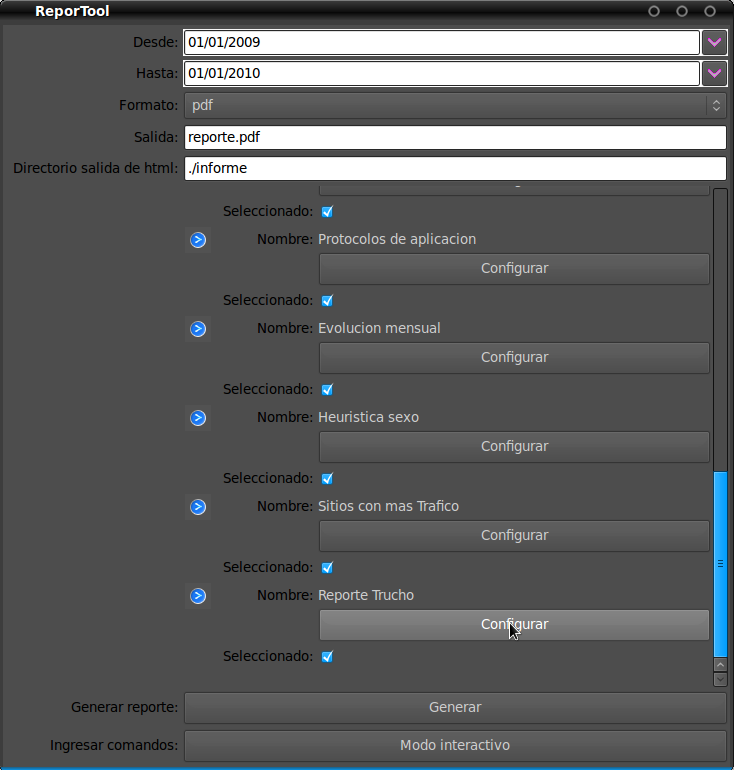
\includegraphics[scale=0.5]{./figuras/reporteAgregado.png}
\end{figure}
\chapter{Instalaci�n y uso}
A continuaci�n daremos una gu�a para realizar la instalaci�n del sniffer y de reporTool. En ambos casos, presentaremos los pasos para un sistema operativo similar a Ubuntu, con python 2.6 ya instalado (por defecto en ubuntu).

\section{Instalaci�n del sniffer}
\begin{enumerate}
\item Instalar easy\_install para python:

\framebox{\begin{minipage}[t][1\totalheight]{1\columnwidth}%
\noindent
\ttfamily
\shorthandoff{"}\\
\hlstd{}\hlsym{$>$\ }\hlstd{sudo\ apt}\hlsym{{-}}\hlstd{get\ }\hlkwc{install\ }\hlstd{python}\hlsym{{-}}\hlstd{setuptools\ python}\hlsym{{-}}\hlstd{dev\ build}\hlsym{{-}}\hlstd{essential}\hspace*{\fill}\\
\mbox{}
\normalfont
\shorthandon{"}
\end{minipage}}

\item Instalar scapy:
 
\framebox{\begin{minipage}[t][1\totalheight]{1\columnwidth}%
\noindent
\ttfamily
\shorthandoff{"}\\
\hlstd{}\hlsym{$>$\ }\hlstd{sudo\ easy\textunderscore install\ scapy}\hspace*{\fill}\\
\mbox{}
\normalfont
\shorthandon{"}
\end{minipage}}


Si esto falla, instala scapy con apt-get (minimo la versi�n 2):

\framebox{\begin{minipage}[t][1\totalheight]{1\columnwidth}%
\noindent
\ttfamily
\shorthandoff{"}\\
\hlstd{}\hlsym{$>$\ }\hlstd{sudo\ apt}\hlsym{{-}}\hlstd{get\ }\hlkwc{install\ }\hlstd{scapy}\hspace*{\fill}\\
\mbox{}
\normalfont
\shorthandon{"}
\end{minipage}}


\item Instalar sqlAlchemy (ORM para la base de datos):

\framebox{\begin{minipage}[t][1\totalheight]{1\columnwidth}%
\noindent
\ttfamily
\shorthandoff{"}
\hlstd{}\hlsym{$>$\ }\hlstd{sudo\ easy\textunderscore install\ sqlalchemy}\hspace*{\fill}\\
\mbox{}
\normalfont
\shorthandon{"}
\end{minipage}}

\item Instalar dpkt (Armado y manipulaci�n de paquetes para varios protocolos), para ello, extraerlo, pararse en el directorio y ejecutar:

\framebox{\begin{minipage}[t][1\totalheight]{1\columnwidth}%
\noindent
\ttfamily
\shorthandoff{"}
\hlstd{}\hlsym{$>$\ }\hlstd{sudo\ python\ setup.py\ }\hlkwc{install}\hlstd{}\hspace*{\fill}\\
\mbox{}
\normalfont
\shorthandon{"}
\end{minipage}}

\item En la versi�n de scapy que bajamos nosotros hay un bug que impide cargar correctamente un archivo pcap. Nosotros hicimos un bugfix de eso, y se encuentra en la carpeta bugfix del CD. Para utilizarlo hay que reemplazar el archivo \verb_/var/lib/python-support/python2.6/sccapy/utils.py_ por el que brindamos nosotros.

\end{enumerate}

\section{Uso del sniffer}
Antes de empezar a sniffear hay que crear la base de datos para que el sniffer pueda guardar los paquetes. Para eso basta con ejecutar:

\framebox{\begin{minipage}[t][1\totalheight]{1\columnwidth}%
\noindent
\ttfamily
\shorthandoff{"}
\hlstd{}\hlsym{$>$\ }\hlstd{python\ persistencia.py}\hspace*{\fill}\\
\mbox{}
\normalfont
\shorthandon{"}
\end{minipage}}

Una vez hecho esto, ya se puede correr el sniffer con:

\framebox{\begin{minipage}[t][1\totalheight]{1\columnwidth}%
\noindent
\ttfamily
\shorthandoff{"}
\hlstd{}\hlsym{$>$\ }\hlstd{sudo\ python\ sniff.py}\hspace*{\fill}\\
\mbox{}
\normalfont
\shorthandon{"}
\end{minipage}}

Las opciones que soporta el sniffer son:
\begin{itemize}
\item -p nroPuerto (--port nroPuerto): Setea el puerto del proxy al valor nroPuerto. Por defecto es 8080
\item -i IP (--ip IP): Setea la ip del proxy al valor IP. Por defecto se ignora la ip, y se asume que todo trafico al puerto del proxy, va para el proxy.
\item -d file (--dump file): Guardar la sesi�n de sniffeo en un archivo pcap de nombre file.
\item -v (--verbose): Modo verbose, se muestra un resumen de cada paquete (a nivel tcp) que captura el sniffer.
\item -f file (--from-file file): Realizar la sesi�n simulando que se sniffean los paquetes que estan en el archivo pcap file
\item -h (--help): Mostrar ayuda, con las posibles opciones que tiene el sniffer
\end{itemize}

Una vez lanzado el sniffer continua corriendo, hasta que se lo interrumpa con \textit{ctrl+c}

\section{Instalaci�n de reporTool}

\section{Uso de reporTool}
ReporTool se puede ejecutar dandole permisos de ejecuci�n a reporTool.py y haciendo doble click en el, o sino desde una consola corriendo:

\framebox{\begin{minipage}[t][1\totalheight]{1\columnwidth}%
\noindent
\ttfamily
\shorthandoff{"}
\hlstd{}\hlsym{$>$\ }\hlstd{python\ reporTool.py}\hspace*{\fill}\\
\mbox{}
\normalfont
\shorthandon{"}
\end{minipage}}

Una vez abierta la interfaz grafica, la misma presenta:
\begin{itemize}
\item Desde: Fecha a partir de la cual se tienen en cuenta los mensajes HTTP para hacer los reportes
\item Hasta: Fecha hasta la cual se tienen en cuenta los mensajes HTTP para hacer los reportes
\item Formato de salida: Puede ser PDF, HTML, o ambos.
\item Salida: Nombre del archivo PDF a generar (si se escogi� PDF o ambos)
\item Directorio salida de html: Nombre del directorio donde crear el reporte HTML (si se escogi� HTML o ambos)
\item Lista con los reportes disponibles. Cada uno puede ser seleccionado y configurado.
\item Generar: Dispara la generaci�n de los reportes seleccionados
\item Modo interactivo: Abre una consola python, como se coment� anteriormente
\end{itemize}


\chapter{Conclusiones}
\label{LastPage}
\end{document}
